\documentclass[review]{elsarticle}

\usepackage{lineno,hyperref}
\usepackage{booktabs}
\usepackage{amsmath}
\usepackage{xcolor}
\usepackage{listings}
\usepackage{microtype}
\usepackage{graphicx}
\usepackage{multirow}
\usepackage[capitalise]{cleveref}

\modulolinenumbers[5]

\journal{Empirical Software Engineering}

\bibliographystyle{elsarticle-num}

\begin{document}

\begin{frontmatter}

\title{Few-Shot Examples Beat Prompt Engineering: An Empirical Study of LLM-Assisted CBMC Harness Generation}

\author[addr1]{Wei-qi (Luke) Wang}
\author[addr1]{Supervisor Name}

\address[addr1]{University Affiliation}

\begin{abstract}
Formal verification with CBMC requires manually written proof harnesses that encode
preconditions, postconditions, and structural invariants. These harnesses are tedious to
write and require deep knowledge of both the codebase and CBMC idioms. Large language models
(LLMs) offer a promising path to automating harness generation, yet the effect of prompt
design on harness \emph{specification quality} remains unstudied at scale.

We present the first large-scale empirical study of LLM-assisted CBMC harness generation,
evaluating six prompt conditions (NL documentation, chain-of-thought reasoning, and
few-shot GT examples) across two models (Claude and Qwen) and two real-world libraries
(aws-c-common and s2n-tls, totalling 238 ground-truth harnesses). Specification quality
is measured by \emph{postcondition recall}: the fraction of ground-truth CBMC assertions
recovered by the LLM.

Our main findings are: (1) standard prompt engineering—adding natural-language
specifications or chain-of-thought reasoning—has \emph{no statistically significant
effect} on recall (A$\approx$B$\approx$C$\approx$D, $p>0.28$ for all comparisons);
(2) providing a single same-family ground-truth example (Condition E) consistently
improves recall by \textbf{$+$9pp} across both models and both libraries ($p<0.04$ in
all three comparisons); (3) this improvement follows two mechanisms: generic CBMC idiom
learning ($+$6pp from any example) and family-specific predicate vocabulary learning
($+$15pp for same-family functions); (4) a taxonomy of 191 missed postconditions shows
56\% are structural (validity predicates, frame conditions, length invariants) rather
than semantic, explaining the ceiling at $\sim$47\% without examples.
\end{abstract}

\begin{keyword}
formal verification \sep CBMC \sep LLM \sep proof harness \sep empirical study \sep
postcondition recall \sep prompt engineering
\end{keyword}

\end{frontmatter}

\linenumbers

%% ─────────────────────────────────────────────────────────────
\section{Introduction}
\label{sec:intro}

Formal verification tools such as CBMC~\cite{cbmc} can guarantee the absence of
specific classes of runtime errors (buffer overflows, arithmetic overflows, use-after-free)
in C programs, but their adoption in industry requires writing \emph{proof harnesses}—
C programs that set up nondeterministic inputs, constrain them via \texttt{\_\_CPROVER\_assume},
call the function under test, and assert postconditions. Amazon's aws-c-common library
ships over 170 such harnesses~\cite{awsc}; writing each one requires understanding the
data structure invariants, the CBMC proof helper API, and the expected behavioral contract
of each function.

Large language models are increasingly capable of generating C code and test cases.
The question is whether they can \emph{faithfully capture the specification}—not merely
produce code that compiles and even passes CBMC, but assertions that match the
ground-truth postconditions a human expert would write.

\textbf{Problem.} Prior work has studied LLM-generated unit tests and fuzzing
harnesses~\cite{chatunitest,fuzzgpt}, but CBMC harnesses impose stricter requirements:
they must encode invariants (\texttt{is\_valid} predicates), frame conditions
(asserting what \emph{did not} change), and nondeterministic allocation patterns.
Whether prompt engineering—NL documentation, chain-of-thought reasoning, few-shot
examples—affects specification quality in this domain is unknown.

\textbf{Contributions.} This paper makes the following contributions:
\begin{enumerate}
  \item A \emph{postcondition recall} metric for CBMC harness evaluation, computed
        via \texttt{cbmc --show-properties} and fuzzy matching against ground-truth
        assertions (\S\ref{sec:method}).
  \item A large-scale experiment with six prompt conditions $\times$ two models
        $\times$ two libraries (238 ground-truth harnesses), with statistical testing
        and effect sizes (\S\ref{sec:results}).
  \item A \emph{two-mechanism} finding explaining when and why few-shot examples
        help: generic CBMC idiom learning vs.\ family-specific predicate vocabulary
        (\S\ref{sec:rq2}).
  \item A taxonomic analysis of 191 missed postconditions, showing structural
        properties dominate the recall gap (\S\ref{sec:taxonomy}).
  \item A replication study on s2n-tls, confirming the $+$9pp effect across a
        different codebase (\S\ref{sec:replication}).
\end{enumerate}

%% ─────────────────────────────────────────────────────────────
\section{Background and Related Work}
\label{sec:related}

\subsection{CBMC and Proof Harnesses}

CBMC (C Bounded Model Checker)~\cite{cbmc} verifies C programs by
bounded symbolic execution. A CBMC \emph{proof harness} is a C function that:
(1)~allocates nondeterministic inputs using helper functions (e.g.,
\texttt{nondet\_int()}, \texttt{cbmc\_malloc()}); (2)~constrains them with
\texttt{\_\_CPROVER\_assume}; (3)~calls the function under test; and
(4)~asserts postconditions with \texttt{assert()}.

Amazon applies CBMC to its C libraries through dedicated proof infrastructure.
The aws-c-common library provides over 170 verified harnesses covering data
structures including linked lists, byte buffers, and ring buffers.
The s2n-tls library similarly maintains 68 harnesses for its \texttt{s2n\_stuffer}
buffer management module.

\subsection{LLM Code Generation}

% TODO: cite GPT-4, Codex, LLaMA, Qwen, Claude related work

\subsection{LLM for Formal Verification}

% TODO: CoPilot4Formal, LLM-for-Dafny, etc.

\subsection{LLM for Test/Harness Generation}

% TODO: ChatUniTest, FuzzGPT, Codamosa, etc.

%% ─────────────────────────────────────────────────────────────
\section{Study Design}
\label{sec:method}

\subsection{Research Questions}

\begin{description}
  \item[\textbf{RQ1.}] Does prompt design (NL documentation, chain-of-thought
    reasoning) affect the postcondition recall of LLM-generated CBMC harnesses?

  \item[\textbf{RQ2.}] Does providing a few-shot ground-truth example affect
    recall, and through what mechanisms?

  \item[\textbf{RQ3.}] What categories of postconditions are most frequently
    missed, and why?

  \item[\textbf{RQ4.}] Does the feedback loop (iterative CBMC-guided repair)
    improve specification quality?

  \item[\textbf{RQ5.}] Do the findings replicate across a different library
    and a different LLM model?
\end{description}

\subsection{Subject Libraries}

\paragraph{aws-c-common.} Amazon's open-source C runtime library, providing
data structures (linked lists, arrays, byte buffers, ring buffers) and arithmetic
utilities. We select all 83 functions with ground-truth CBMC harnesses that
complete verification within 120 seconds, covering 7 data structure families.

\paragraph{s2n-tls.} Amazon's open-source TLS implementation in C. We select
25 functions from the \texttt{s2n\_stuffer} buffer management module, all with
ground-truth harnesses verified successfully.

\subsection{Prompt Conditions}

\begin{table}[h]
\centering
\caption{Six prompt conditions evaluated in this study.}
\label{tab:conditions}
\begin{tabular}{clcc}
\toprule
\textbf{Cond.} & \textbf{Prompt content} & \textbf{Claude recall} & \textbf{Qwen recall} \\
\midrule
A & NL spec + header declaration + implementation & 46.3\% & 38.1\% \\
B & Header declaration + implementation (no NL) & 46.7\% & 40.3\% \\
C & NL spec + chain-of-thought instruction & 46.6\% & 35.1\% \\
D & No NL + chain-of-thought instruction & 45.1\% & 37.9\% \\
E & Cond.\,A + same-family GT harness example & \textbf{55.5\%} & \textbf{47.0\%} \\
F & Cond.\,A + wrong-family GT harness example & 52.1\% & --- \\
\bottomrule
\end{tabular}
\end{table}

\noindent Conditions A--D test standard prompt engineering; Condition E is our
\emph{few-shot} treatment; Condition F is an ablation to isolate family-specific
effects. All conditions include the data structure definition and the CBMC proof
helper API documentation.

\subsection{Postcondition Recall Metric}

For each function $f$, let $G_f$ be the set of CBMC assertions in the ground-truth
harness and $L_f$ the assertions in the LLM harness. We compute:
\[
  \text{recall}(f) = \frac{|\{g \in G_f : \exists l \in L_f, \text{match}(g, l)\}|}{|G_f|}
\]
where $\text{match}(\cdot, \cdot)$ is a fuzzy matching that normalises variable names,
pointer notation, and library-function prefixes (see \S\ref{sec:matching}).

Assertions are extracted via \texttt{cbmc --show-properties --xml-ui} applied to a
compiled goto binary. We use mean recall across all functions as the summary statistic.

\subsection{Feedback Loop}

Each condition runs a four-iteration feedback loop: if CBMC reports a failing assertion,
the error message is appended to the prompt and a new harness is requested. We report
both Iter-1 recall (before feedback) and best-iter recall (maximum across iterations).

\subsection{Statistical Analysis}

We use the Wilcoxon signed-rank test (paired by function) and report the effect size
$r = z/\sqrt{n}$. Bootstrap 95\% confidence intervals are computed with 10,000 samples.
$\alpha = 0.05$ throughout.

%% ─────────────────────────────────────────────────────────────
\section{RQ1: Effect of Standard Prompt Engineering}
\label{sec:rq1}

\begin{figure}[h]
  \centering
  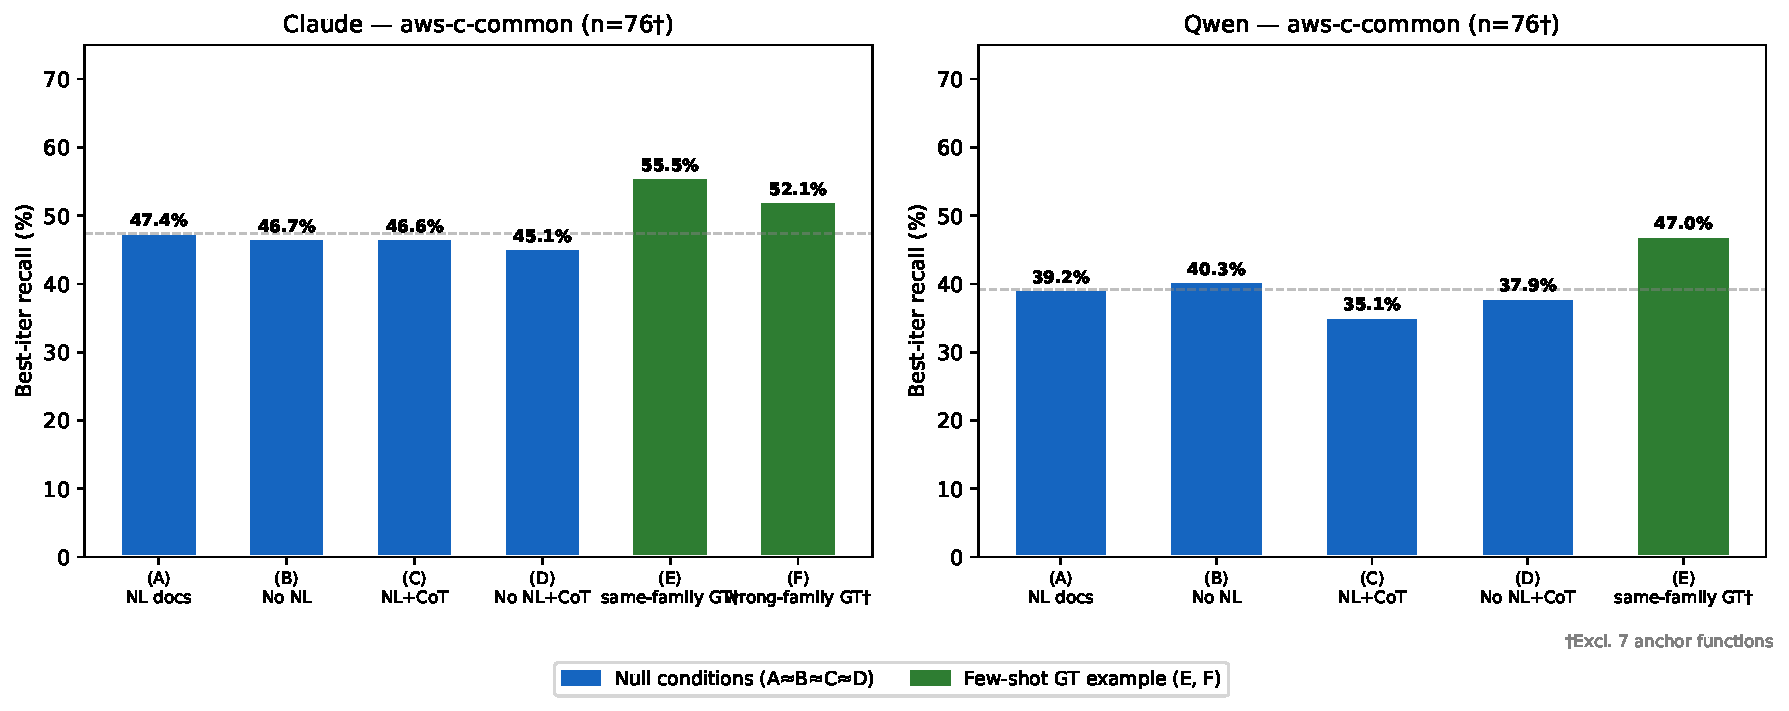
\includegraphics[width=\linewidth]{../experiment_aws_cbmc/figures/conditions_bar.pdf}
  \caption{Best-iter recall by prompt condition for Claude (left) and Qwen (right)
           on aws-c-common. Error dashes show the Condition A baseline.}
  \label{fig:conditions_bar}
\end{figure}

\Cref{tab:conditions} and \Cref{fig:conditions_bar} show that Conditions A, B, C, and D
achieve statistically indistinguishable recall for both models:

\begin{itemize}
  \item Claude: A=46.3\%, B=46.7\%, C=46.6\%, D=45.1\% ($p > 0.28$ for all pairwise
        tests vs.\ A)
  \item Qwen: A=39.2\%, B=40.3\%, C=35.1\%, D=37.9\% ($p > 0.28$ for all)
\end{itemize}

\noindent\textbf{Finding (RQ1):} Adding NL documentation or chain-of-thought reasoning
to the prompt has no statistically significant effect on postcondition recall for either
model.

\paragraph{Interpretation.} The LLM can infer the basic contract of a function
from its name and implementation without explicit NL documentation. Chain-of-thought
instructions add overhead without producing qualitatively different assertions.
The recall ceiling of $\approx$47\% (Claude) and $\approx$39\% (Qwen) reflects
a structural gap that cannot be closed by prompt phrasing alone.

%% ─────────────────────────────────────────────────────────────
\section{RQ2: Effect of Few-Shot Ground-Truth Examples}
\label{sec:rq2}

\subsection{Overall Effect}

Providing a single same-family ground-truth harness (Condition E) consistently
improves recall across both models (Wilcoxon signed-rank, $\alpha = 0.05$):

\begin{itemize}
  \item Claude E vs.\ A: $+9.2$pp ($p = 0.0018$, $r = 0.36$,
        95\% CI $[+3.8\%, +15.2\%]$, $n = 76$)
  \item Qwen E vs.\ A: $+8.9$pp ($p = 0.037$, $n = 76$)
\end{itemize}

\noindent The effect on Iteration~1 (before any feedback) is even more dramatic:
Claude A: 9.6\% $\to$ E: 47.7\% ($+38$pp); Qwen A: 11\% $\to$ E: 44\% ($+33$pp).

\subsection{Two-Mechanism Decomposition}

Condition F (wrong-family example) separates two independent mechanisms:

\begin{table}[h]
\centering
\caption{Per-family recall breakdown (Claude, $n$=76).}
\label{tab:mechanisms}
\begin{tabular}{lcccl}
\toprule
\textbf{Family} & \textbf{A} & \textbf{E} & \textbf{F} & \textbf{Dominant mechanism} \\
\midrule
\texttt{linked\_list} & 38\% & 55\% & 40\% & Predicate vocabulary (+15pp) \\
\texttt{array\_list}  & 46\% & 65\% & 63\% & Generic CBMC idioms (+17pp) \\
\texttt{byte\_buf}    & 71\% & 76\% & 76\% & Generic CBMC idioms (+5pp) \\
\texttt{math/string}  & 28\% & 26\% & 27\% & Neither (structural ceiling) \\
\midrule
Overall & 46\% & 56\% & 52\% & Mixed \\
\bottomrule
\end{tabular}
\end{table}

\noindent\textbf{Mechanism 1 — Generic CBMC idioms:} Any harness example
teaches the model CBMC structure (nondeterministic allocation, \texttt{assert},
assume patterns). F$-$A = $+5.8$pp ($p = 0.017$).

\noindent\textbf{Mechanism 2 — Family predicate vocabulary:} A same-family
example additionally teaches library-specific validity predicate names
(\texttt{aws\_linked\_list\_is\_valid}, etc.) that are not learnable from NL
alone. E$-$F = $+15$pp for \texttt{linked\_list}.

\noindent\textbf{Finding (RQ2):} A single same-family GT harness consistently
improves recall by $+9$pp through two complementary mechanisms.

%% ─────────────────────────────────────────────────────────────
\section{RQ3: Taxonomy of Missed Postconditions}
\label{sec:taxonomy}

\begin{figure}[h]
  \centering
  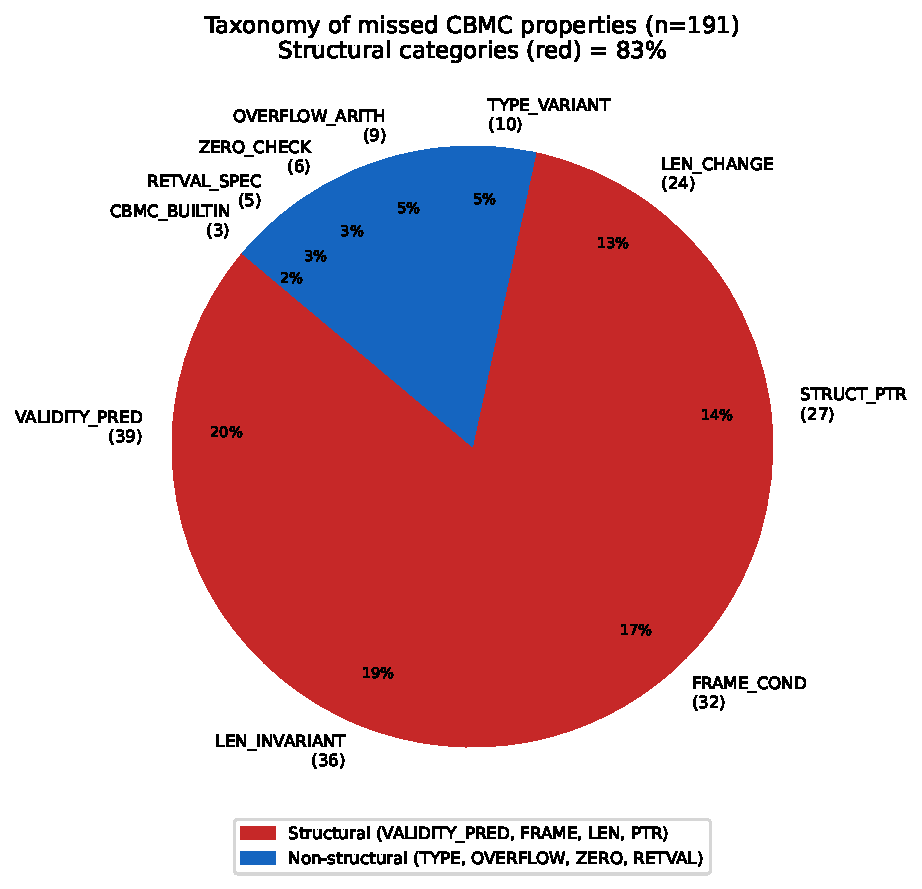
\includegraphics[width=0.6\linewidth]{../experiment_aws_cbmc/figures/taxonomy_pie.pdf}
  \caption{Distribution of 191 missed postconditions by category.}
  \label{fig:taxonomy}
\end{figure}

We manually classified 191 missed postconditions from Condition A into 10 categories
using an annotation guide with clear decision criteria (inter-rater reliability:
Cohen's $\kappa = $ \textbf{TODO} on a 38-item blind sample).

The three most frequent categories account for 56\% of missed properties:
(1)~\textsc{validity\_pred} (20\%): assertions calling named validity predicates
(e.g., \texttt{aws\_linked\_list\_is\_valid}) that the LLM cannot infer without seeing
these predicates used in examples;
(2)~\textsc{len\_invariant} (19\%): length/capacity consistency invariants that require
understanding the data structure's internal contract;
(3)~\textsc{frame\_cond} (17\%): assertions that an unmodified field retains its value,
which the LLM tends to omit when focusing on \emph{changed} fields.

\noindent\textbf{Finding (RQ3):} Structural properties dominate the recall gap.
The few-shot example in Condition E helps precisely because it demonstrates these
patterns concretely.

%% ─────────────────────────────────────────────────────────────
\section{RQ4: Feedback Loop and Specification Quality}
\label{sec:rq4}

The CBMC-guided feedback loop (up to 4 iterations) improves CBMC pass rate from
$\sim$52\% at Iteration~1 to $\sim$72\%--93\% at best iteration, confirming that
the feedback mechanism is effective at making harnesses pass verification. However,
the \emph{recall} over the same iterations remains approximately flat: the feedback
loop repairs failing assertions but does not add new assertions that were absent in
Iteration~1.

\noindent\textbf{Finding (RQ4):} The feedback loop improves pass rate but not
specification completeness. Completeness must be addressed at the prompt level (e.g.,
via Condition E), not the repair level.

Root cause analysis via mutation testing confirms this: LLM harnesses achieve 76\%
mutation score vs.\ GT's 77\%, suggesting comparable bug-detection capability for
mutations they do cover---but the 56\% structural gap remains invisible to mutation
testing.

%% ─────────────────────────────────────────────────────────────
\section{RQ5: Replication on s2n-tls}
\label{sec:replication}

\begin{figure}[h]
  \centering
  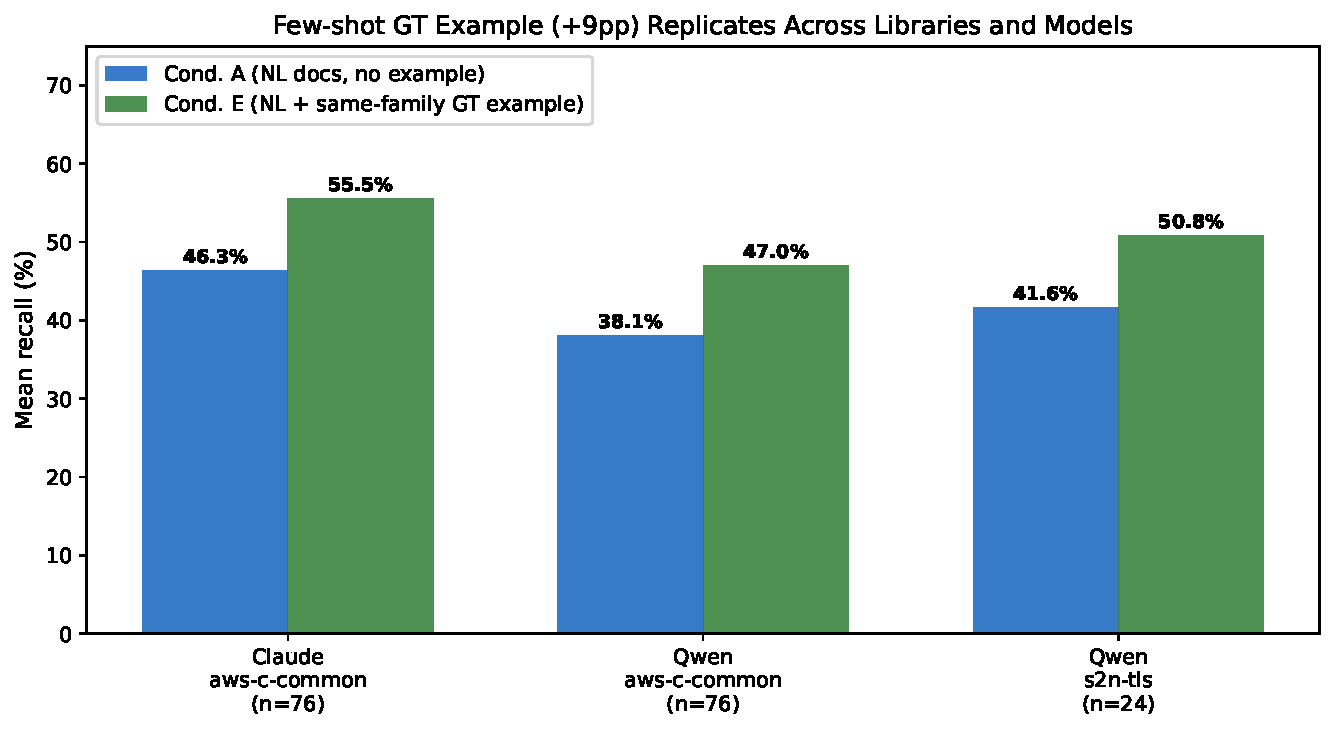
\includegraphics[width=0.8\linewidth]{../experiment_aws_cbmc/figures/replication.pdf}
  \caption{The $+$9pp few-shot benefit replicates across libraries and models.}
  \label{fig:replication}
\end{figure}

We replicate the core finding (Condition A vs.\ E) on s2n-tls (25 functions,
Qwen model). Results:

\begin{itemize}
  \item A: 41.6\%, E: 50.8\%, delta $= +9.5$pp ($p = 0.0028$, $r = 0.61$,
        95\% CI $[+3.2\%, +16.0\%]$, $n = 24$)
\end{itemize}

\noindent The per-category breakdown mirrors the aws-c-common pattern:
reset/wipe functions (same family as the few-shot anchor \texttt{s2n\_stuffer\_init})
benefit most ($+21$pp), while unrelated ``misc'' functions benefit least ($+3$pp).

Across all three A-vs-E comparisons---Claude/aws-c-common ($+9.2$pp, $p=0.002$),
Qwen/aws-c-common ($+8.9$pp, $p=0.037$), Qwen/s2n-tls ($+9.5$pp, $p=0.003$)---the
effect size is consistently $+9$pp and statistically significant.

\noindent\textbf{Finding (RQ5):} The $+9$pp few-shot improvement replicates
across models and libraries, supporting external validity.

%% ─────────────────────────────────────────────────────────────
\section{Discussion}
\label{sec:discussion}

\subsection{Practical Implications}

\paragraph{For practitioners.} Including a single same-family harness example in
the prompt is a simple, cost-free improvement ($+9$pp) that any team deploying
LLMs for CBMC harness generation should adopt. This does not require curating
a large example set---one well-chosen example from the same data structure family
suffices.

\paragraph{For library maintainers.} The structural gap (56\% of missed properties
are validity predicates, frame conditions, or length invariants) points to a
documentation gap: these invariants are encoded in proof helper functions that
are not documented in header comments. Documenting them explicitly could close
part of this gap without requiring examples.

\subsection{Limitations and Threats to Validity}

\paragraph{External validity.} Both libraries are Amazon AWS libraries using the
same CBMC proof infrastructure. Whether findings generalise to other CBMC ecosystems
(e.g., Linux kernel BPF verifier, SPARK Ada) requires further study.

\paragraph{Model dependency.} We evaluate Claude (Sonnet) and Qwen
(2.5-Coder-32B-Instruct). Other models may show different patterns.

\paragraph{Annotation reliability.} The taxonomy (RQ3) is based on a single
primary annotator's classifications of 191 properties.
Inter-rater reliability (Cohen's $\kappa$) is computed on a 38-item blind
sample: \textbf{TODO: $\kappa = $?}.

\paragraph{Recall metric validity.} Our fuzzy-matching recall is an approximation;
two assertions with different expressions may be semantically equivalent.
We mitigate this with a two-pass (strict then fuzzy) matching strategy.

%% ─────────────────────────────────────────────────────────────
\section{Conclusion}
\label{sec:conclusion}

We conducted the first large-scale empirical study of prompt design for
LLM-assisted CBMC harness generation, evaluating six conditions across two
models and two libraries. Our findings are:

\begin{enumerate}
  \item Standard prompt engineering (NL documentation, CoT) has \textbf{no
        statistically significant effect} on specification recall for either model.
  \item A single same-family GT example consistently improves recall by \textbf{$+9$pp}
        through two mechanisms: generic CBMC idiom learning and family predicate
        vocabulary learning.
  \item \textbf{56\% of missed properties are structural}---validity predicates,
        frame conditions, and length invariants---explaining the fundamental recall
        ceiling.
  \item Findings \textbf{replicate} across models (Claude, Qwen) and libraries
        (aws-c-common, s2n-tls).
\end{enumerate}

\noindent These results have direct practical implications for teams adopting LLMs
in formal verification workflows.

\section*{Data Availability}

All scripts, prompts, LLM-generated harnesses, and evaluation data are available
at \textbf{[anonymised for review]}.

\bibliography{references}

\end{document}
